\onecolumn
\section{Appendice}

\subsection{Graphs}
\label{ssec:graphs}

\begin{figure}[H]
  \caption{Memory Usage whilst executing the algorithm 1000000 times.}
  \label{grf:mem-usage}
  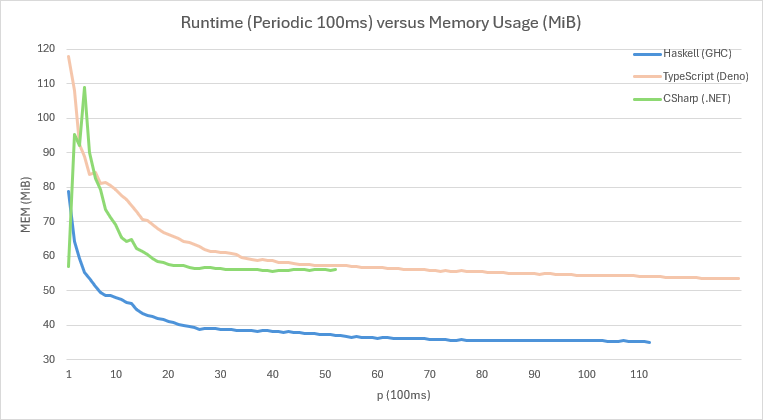
\includegraphics[width=0.5\textwidth]{./img/mem-usage.png}
\end{figure}


\begin{figure}[H]
  \caption{CPU Usage whilst executing the algorithm 1000000 times.}
  \label{grf:cpu-usage}
  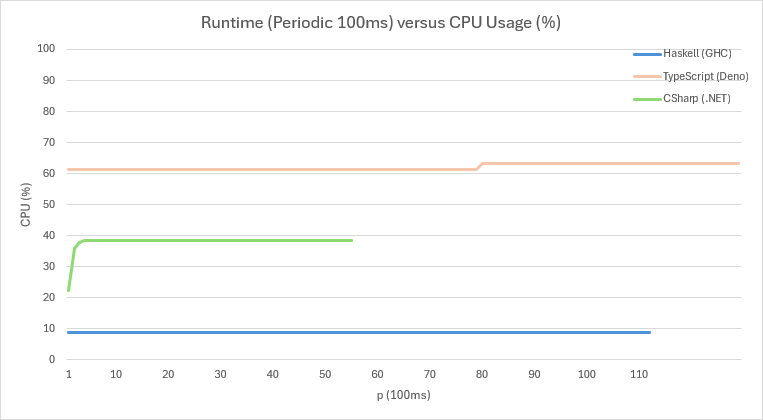
\includegraphics[width=0.5\textwidth]{./img/cpu-usage.png}
\end{figure}

\begin{landscape}
\subsection{Benchmark Summaries}
\label{ssec:benchmark-s}
\begin{figure}[H]
  \caption{Benchmark results for the TypeScript implementation using the Deno runtime.}
  \label{code:benchmark-typescript}
  \begin{minted}[fontsize=\footnotesize]{text}
  CPU | AMD Ryzen 5 5600X 6-Core Processor
  Runtime | Deno 2.0.0 (x86_64-unknown-linux-gnu)

  benchmark                                           time/iter (avg)        iter/s      (min … max)           p75      p99     p995
  --------------------------------------------------- ----------------------------- --------------------- --------------------------
  levenshteinRatio - short identical strings                   5.1 ns   195,400,000 (  5.0 ns …  24.6 ns)   5.0 ns   7.5 ns   9.2 ns
  levenshteinRatio - short different strings                 144.9 ns     6,904,000 (137.0 ns … 182.7 ns) 148.7 ns 173.1 ns 182.5 ns
  levenshteinRatio - short similar strings                   323.3 ns     3,093,000 (299.4 ns … 613.6 ns) 325.8 ns 465.5 ns 613.6 ns
  levenshteinRatio - long identical strings                    5.3 ns   187,100,000 (  5.1 ns … 145.6 ns)   5.1 ns   7.9 ns   9.0 ns
  levenshteinRatio - long different strings                    7.0 ms         142.0 (  6.5 ms …  12.3 ms)   6.9 ms  12.3 ms  12.3 ms
  levenshteinRatio - long partially similar strings            7.5 ms         133.6 (  7.2 ms …   8.1 ms)   7.6 ms   8.1 ms   8.1 ms
  \end{minted}
\end{figure}

\hfill

\begin{figure}[H]
  \caption{Benchmark results for the C\# implementation using BenchmarkDotNet.}
  \label{code:benchmark-csharp}
  \begin{minted}[fontsize=\footnotesize]{text}
  Runtime = .NET 9.0.3 (9.0.325.11113), X64 RyuJIT AVX2; GC = Concurrent Workstation
  Mean = 3.233 ms, StdErr = 0.004 ms (0.14%), N = 14, StdDev = 0.017 ms
  Min = 3.204 ms, Q1 = 3.221 ms, Median = 3.233 ms, Q3 = 3.246 ms, Max = 3.259 ms
  IQR = 0.025 ms, LowerFence = 3.184 ms, UpperFence = 3.283 ms
  ConfidenceInterval = [3.214 ms; 3.252 ms] (CI 99.9%), Margin = 0.019 ms (0.59% of Mean)
  Skewness = -0.19, Kurtosis = 1.65, MValue = 2

  BenchmarkDotNet v0.14.0, Debian GNU/Linux 12 (bookworm) (container)
  AMD Ryzen 5 5600X, 1 CPU, 12 logical and 6 physical cores
  .NET SDK 9.0.201

  | Method                      | Mean             | Error          | StdDev         |
  |---------------------------- |-----------------:|---------------:|---------------:|
  | ShortIdenticalStrings       |         1.410 ns |      0.0510 ns |      0.0793 ns |
  | ShortDifferentStrings       |       112.147 ns |      1.4472 ns |      1.3537 ns |
  | ShortSimilarStrings         |       193.013 ns |      1.8653 ns |      1.7448 ns |
  | LongIdenticalStrings        |         1.097 ns |      0.0221 ns |      0.0196 ns |
  | LongDifferentStrings        | 3,234,542.032 ns | 34,662.1297 ns | 32,422.9776 ns |
  | LongPartiallySimilarStrings | 3,233,473.960 ns | 18,980.6706 ns | 16,825.8701 ns |

    Mean   : Arithmetic mean of all measurements
    Error  : Half of 99.9% confidence interval
    StdDev : Standard deviation of all measurements
    1 ns   : 1 Nanosecond (0.000000001 sec)

  Run time: 00:02:27 (147.1 sec), executed benchmarks: 6

  Global total time: 00:03:08 (188.25 sec), executed benchmarks: 6
  \end{minted}
\end{figure}
\hfill

\begin{figure}[H]
  \caption{Benchmark results for the Haskell implementation using Criterion.}
  \label{code:benchmark-haskell}
  \begin{minted}[fontsize=\footnotesize]{text}
  benchmarking levenshteinRatio - short identical strings
  time                 20.15 ns   (19.87 ns .. 20.38 ns)
                       0.999 R²   (0.998 R² .. 0.999 R²)
  mean                 20.15 ns   (20.00 ns .. 20.36 ns)
  std dev              604.4 ps   (497.4 ps .. 753.7 ps)

  benchmarking levenshteinRatio - short different strings
  time                 966.6 ns   (953.2 ns .. 985.3 ns)
                       0.996 R²   (0.991 R² .. 0.999 R²)
  mean                 992.3 ns   (970.7 ns .. 1.036 us)
  std dev              97.98 ns   (50.78 ns .. 187.7 ns)

  benchmarking levenshteinRatio - short similar strings
  time                 2.410 us   (2.386 us .. 2.436 us)
                       0.999 R²   (0.999 R² .. 1.000 R²)
  mean                 2.391 us   (2.374 us .. 2.417 us)
  std dev              69.63 ns   (50.30 ns .. 104.4 ns)

  benchmarking levenshteinRatio - long identical strings
  time                 3.786 us   (3.765 us .. 3.815 us)
                       1.000 R²   (0.999 R² .. 1.000 R²)
  mean                 3.815 us   (3.795 us .. 3.842 us)
  std dev              79.62 ns   (63.85 ns .. 103.2 ns)

  benchmarking levenshteinRatio - long different strings
  time                 1.178 s    (847.8 ms .. 1.411 s)
                       0.991 R²   (0.970 R² .. 1.000 R²)
  mean                 1.174 s    (1.121 s .. 1.245 s)
  std dev              68.38 ms   (32.52 ms .. 85.07 ms)

  benchmarking levenshteinRatio - long partially similar strings
  time                 1.159 s    (816.3 ms .. 1.381 s)
                       0.990 R²   (0.968 R² .. 1.000 R²)
  mean                 1.158 s    (1.120 s .. 1.214 s)
  std dev              53.67 ms   (17.17 ms .. 70.20 ms)
  \end{minted}
\end{figure}
\hfill

\subsection*{Source Code}
\begin{figure}[H]
  \caption{TypeScript implementation of the Levenshtein distance algorithm.}
  \label{code:typescript}
  \inputminted[fontsize=\footnotesize]{typescript}{./doc/levenshteinRatio.ts}
\end{figure}

\hfill

\begin{figure}[H]
  \caption{C\# implementation of the Levenshtein distance algorithm.}
  \label{code:csharp}
  \inputminted[fontsize=\footnotesize]{csharp}{./doc/LevenshteinRatio.cs}
\end{figure}

\hfill

\begin{figure}[H]
  \caption{Haskell implementation of the Levenshtein distance algorithm.}
  \label{code:haskell}
  \inputminted[fontsize=\footnotesize]{haskell}{./doc/LevenshteinRatio.hs}
\end{figure}

\end{landscape}
